\documentclass[conference]{IEEEtran}
\usepackage{graphicx,booktabs,amsmath,array,url}
\usepackage[hidelinks]{hyperref}
\newcommand{\code}[1]{\texttt{\small #1}}
\title{E-Commerce Anomaly Analysis and\\Credit-Card Fraud Benchmarking\\\large ITCS544 Phase 2 Progress Report}
\author{\IEEEauthorblockN{Khon Cho Thar Byin (6837922), Chuchan Ou (6836902), Aye Myo Myat (6837919)}\IEEEauthorblockA{Faculty of Information and Communication Technology, Mahidol University\\12 October 2026}}
\begin{document}\maketitle
\begin{abstract}
We implement and execute a warehouse and preliminary mining pipeline over 5,511,929 REES46 e-commerce events and 284,807 ULB/Worldline credit-card transactions. The second dataset supplies a labeled fraud benchmark without inventing links to the unlabeled clickstream. A six-task Apache Airflow DAG orchestrates deterministic extraction, PySpark staging, a constrained dimensional warehouse, feature preparation, five OLAP benchmarks, and mining. The warehouse contains 1,225,832 visits and 128,525 observed product versions; integrity and temporal checks pass. Five query workloads are evaluated across native storage, secondary indexes, and date-partitioned Parquet. Session clustering and Isolation Forest provide exploratory segmentation and review candidates; on a separate chronological card test set, Random Forest achieves average precision 0.812 and F1 0.820. Results are preliminary and do not establish fraud accuracy for REES46.
\end{abstract}
\begin{IEEEkeywords}data warehouse, SCD Type 2, ETL, OLAP, anomaly detection, credit-card fraud\end{IEEEkeywords}

\section{Scope, Questions, and Phase 2 Status}
The Phase 1 proposal targets unusual e-commerce behavior and session segmentation. This implementation addresses three questions: (RQ1) can a repeatable multi-tier pipeline preserve event/session semantics at more than five million raw records; (RQ2) which physical strategy benefits the required multidimensional queries; and (RQ3) what preliminary anomaly, cluster, and labeled benchmark evidence is supportable? The deliverables follow the Phase 2 assignment: functional warehouse, ERD and bus matrix, executed ETL with quality metrics, five measured OLAP queries, and preliminary mining preparation and baselines [1].

The added ULB/Worldline dataset [3], [4] is relevant because it contains confirmed fraud labels that the proposed REES46 dataset lacks. Both sources are actually loaded and analyzed. They have separate fact grains, separate time semantics, and separate models. Shared source metadata allows one governed project, not an entity-level merge. Neither card labels nor card model accuracy are transferred to clickstream sessions.

\subsection{Implementation decision}
The runnable analytical store uses DuckDB 1.4.3 instead of the proposal's PostgreSQL. The execution environment could not run PostgreSQL under its available account. PySpark 3.5.7 performs typed staging and Apache Airflow 2.10.5 performs orchestration. This is an explicitly documented, single-host analytical prototype; it does not claim PostgreSQL index performance, a distributed deployment, or enterprise availability. A Dockerfile and independent sequential runner support reproduction; the Docker image itself was not built in this environment.

\section{Datasets, Acquisition, and Audit}
\subsection{Original clickstream}
The official REES46 marketplace October 2019 file [2] contains 42,448,764 events. Its nine fields are timestamp, event type, product ID, category ID/code, brand, price, user ID, and source session ID. A deterministic bucket predicate,
\begin{equation}
\operatorname{CRC32}(\text{user ID}\Vert\texttt{|}\Vert\text{session ID})\bmod1000<130,
\end{equation}
selects 5,511,929 events while preserving every available October event belonging to each selected composite source session. Two source rows lack a required session/user identifier and are excluded before selection. Hash selection is repeatable but does not guarantee representativeness for every rare behavior; October boundaries can truncate sessions. The sample alone exceeds the minimum raw-record requirement.

Audited source event types are view (40,779,399), cart (926,516), and purchase (742,849). Although the schema reserves a remove-from-cart category, none occurs in this file. The official catalog spans seven months; the widely cited approximately 285M-event total must not be described as a two-month count. There is no trustworthy order ID, quantity, refund, payment outcome, or confirmed fraud label. Consequently, purchase-event price sums are not settled revenue.

\subsection{Additional labeled source}
The credit-card dataset contains 284,807 transactions and 492 frauds (0.1727\%). It describes approximately two days of European cardholder activity in September 2013. The features are anonymized components V1--V28, elapsed seconds (Time), Amount, and binary Class. We download the exact CSV mirror documented by TensorFlow [4] and record both sources' byte counts and SHA-256 hashes in the acquisition manifest. The card data contains no usable shared customer identifiers or exact calendar timestamps. Time remains elapsed time, and Amount is never added to REES46 price.

\begin{figure}[t]\centering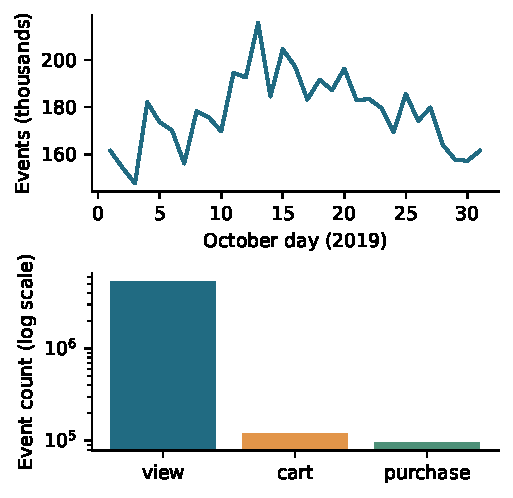
\includegraphics[width=\columnwidth]{eda.pdf}\caption{Selected October event volume and event mix. Counts are observations, not unique orders. The event-type axis uses a logarithmic scale.}\label{fig:eda}\end{figure}
The clickstream is strongly view-dominated; source descriptive fields are incomplete. The card dataset is extremely imbalanced. These properties motivate explicit missingness flags, rate features, temporal evaluation, and precision--recall reporting rather than accuracy alone. Privacy is preserved by retaining pseudonymous identifiers only for joins; no reidentification is attempted. Raw archives are not included in the deliverable. Source attribution, download instructions, and a reminder to check terms before public redistribution accompany the package.

\section{Architecture and Dimensional Modeling}
\subsection{Three tiers and analytical marts}
The raw tier contains immutable downloaded files and a source manifest. The staging tier contains the session-preserving CSV and typed Spark Parquet, with validity and missingness flags. The enterprise warehouse tier contains constrained dimensions and facts; a rejected-row table retains invalid selected records if any arise. The delivery tier provides the five OLAP workloads, a session feature mart, model outputs, and a card evaluation mart. Airflow metadata and JSON/CSV evidence form the execution audit trail.

\begin{figure*}[t]\centering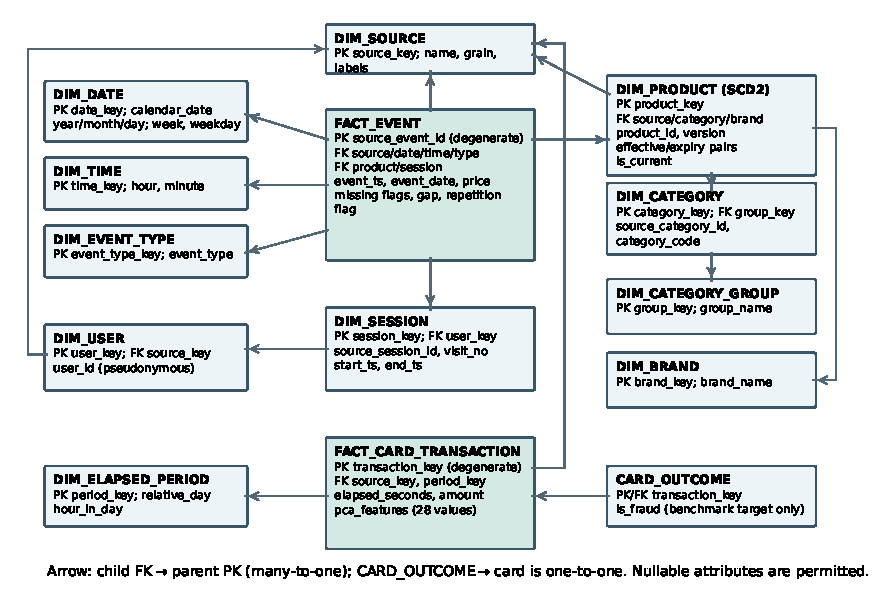
\includegraphics[width=.96\textwidth]{erd.pdf}\caption{Complete core relational ERD. Arrows point from child foreign keys to parent primary keys. The source dimension is shared; the business facts are not joined. Auxiliary tables are documented in the text and executable DDL.}\label{fig:erd}\end{figure*}

\subsection{Grains, keys, and measures}
\textbf{FactEvent} has one row per selected, valid source CSV event, uniquely identified by its original row number in the pinned source file. This source-event key is a degenerate dimension: no artificial order entity is created. Foreign keys reference source, date, minute-of-day, event type, observed product version, and derived visit. Price is decimal(18,2), timestamps are parsed in UTC, IDs are 64-bit integers, and quality flags remain explicit.

\textbf{FactCardTransaction} has one row per source transaction row, with a deterministic row key, source and elapsed-period keys, elapsed seconds, amount, and 28 numeric PCA values. \textbf{CardOutcome} has a one-to-one primary/foreign key relationship with this fact and stores the binary target separately from the feature vector. This reduces accidental label leakage during feature extraction. No exact card date or customer dimension is fabricated.

\textbf{DimSession} has one row per derived visit. Within each (user, source-session) key, a gap strictly greater than 1,800 seconds starts a new visit. Exactly 1,800 seconds remains in the same visit. The 1,201,148 selected source-session keys become 1,225,832 visits. A visit belongs to one user; this is a dimension relationship, not a many-to-many bridge. Source-session IDs and visit sequence numbers are retained for lineage. Unknown source descriptions are mapped to explicit members rather than removing events.

\subsection{Observed product SCD Type 2}
A new product version is created when observed category ID, category code, or brand differs from the previous observation for that product. Events are ordered by (timestamp, source row). The half-open validity interval uses both fields, so simultaneous changes have deterministic ownership. The fact references the matching version; exactly one version per product is current. There are 126,005 products, 128,525 versions, and 2,450 products with more than one observed version.

These are changes in observed descriptive state, not independently verified business master-data changes. Alternation between known and unknown descriptions can create a version. The history reflects the selected sample, not every source event. A full refresh sorts the available history again, so late source observations are reconciled on rebuild; this is not an incremental late-arrival service. No product versions are created merely because event price changes.

\begin{table}[t]\centering\caption{Warehouse bus matrix (X: applicable; --: not applicable)}\label{tab:bus}\scriptsize
\resizebox{\columnwidth}{!}{\begin{tabular}{lccccccc}\toprule
Process & Source & Date/time & Product & Category/brand & Visit/user & Elapsed & Label\\\midrule
Clickstream & X & X & X & X & X & -- & --\\
Card payment & X & -- & -- & -- & -- & X & X\\
Session mart & X & X & X & X & X & -- & --\\\bottomrule
\end{tabular}}\end{table}
The category hierarchy is snowflaked: product version $\rightarrow$ category $\rightarrow$ top-level category group, with brand as a separate dimension. The session mart derives aggregates through those relationships; its product/category applicability does not imply a single product foreign key at session grain. The calendar dimension supports year/month/day and ISO week; minute-of-day supports hourly drill-down. All warehouse fact foreign keys and primary keys are enforced. Auxiliary \code{metadata\_measure} records source-specific definitions; \code{rejected\_events} preserves quarantine rows; \code{session\_features} is a derived mart, not an independent business fact. The external partitioned-event view is a physical replica of FactEvent, not another logical grain.

\section{Executed ETL and Validation}
\subsection{Automation and restart behavior}
The six Airflow tasks are extraction, Spark staging, warehouse build/validation, feature mart, OLAP benchmark, and mining. The complete DAG was executed with Airflow's local \code{dag.test()} facility; this runs real task code and writes metadata but does not demonstrate a continuously running scheduler or multiworker executor. The run status and per-task completion timestamps are included in \code{airflow\_status.json}. Every task completed successfully. The DAG is manual, has one active run, and allows one retry after five seconds.

Extraction scans the original archive and selects whole composite sessions; source row numbers remain stable across replay. Spark validates schema, timestamp, identifiers, nonnegative price, and event vocabulary. It preserves absent descriptions as Unknown and adds missingness indicators. Invalid rows are quarantined rather than silently discarded. SQL creates deterministic surrogate keys, observed SCD histories, visits, and constrained facts. The warehouse is built as a separate snapshot, checked, checkpointed, and then replaces the prior snapshot. Rebuilds must run without concurrent readers/writers. This approach is repeat-idempotent for the pinned files, rather than append-based incremental loading.

\begin{table}[t]\centering\caption{Measured quality before and after processing}\label{tab:quality}\small
\begin{tabular}{p{.44\columnwidth}rr}\toprule
Check & Before & After\\\midrule
Selected clickstream rows & 5,511,929 & 5,511,929\\
Missing brand description & 792,473 & 0 raw nulls$^a$\\
Missing category description & 1,755,280 & 0 raw nulls$^a$\\
Invalid selected rows & 0 & 0 quarantined\\
Exact observed repeat rows$^b$ & 4,063 & 4,063 retained\\
Zero-price events & 9,015 & 9,015 retained\\
Orphan product/session keys & -- & 0 / 0\\
Duplicate event row keys & -- & 0\\
Invalid SCD assignments & -- & 0\\
Products without one current row & -- & 0\\
Card missing feature rows & 0 & 0\\
Card negative amounts & 0 & 0\\\bottomrule
\end{tabular}
\begin{flushleft}\scriptsize $^a$Replaced by Unknown; original missingness remains flagged. $^b$Excess rows in identical observed event groups, excluding the source-row identifier.\end{flushleft}\end{table}
Missing brand and category descriptions affect 14.38\% and 31.85\% of selected events, respectively. Imputation improves join completeness, not source knowledge. Zero prices can reflect free items or recording conventions, so they are preserved. Card Amount contains 1,825 zeros, which are also preserved.

\subsection{Deduplication and anomaly policy}
No upstream event ID proves that identical observed rows are retries. Removing them would erase potentially meaningful rapid-repeat behavior. Therefore the pipeline distinguishes technical duplicate ingestion from observed repetition: the source-row primary key prevents duplicate ingestion on replay, while 4,063 identical observed excess rows are retained. A narrower consecutive same-product/same-type/same-second flag marks 4,047 events. Its definition differs from exact-row duplication and does not assert fraud.

The card source has 1,081 repeated feature rows including elapsed time; these remain distinct source records. Temporal split boundaries keep identical elapsed-time groups together. A future sensitivity analysis should quantify the impact of removing exact duplicates; this preliminary report does not claim independence between all transactions. Quality gates also check that engineered velocity and entropy are finite. Singleton gap standard deviations are filled with zero only in the modeling matrix, with zero meaning no observed gap variation.

\subsection{Measured execution evidence}
The automated extraction scan took 113.1 seconds (download time excluded because the pinned originals were already present); Spark staging took 31.6 seconds; the warehouse build and validation took 60.5 seconds; feature preparation took 4.1 seconds; and both-source mining took 46.7 seconds. The full six-task Airflow run completed in 277.4 seconds, including orchestration and benchmark overhead. These are measured elapsed times on this host, not distributed-throughput claims.
The initial and automated repeat builds both produced 5,511,929 events, 284,807 cards, 492 fraud labels, 1,225,832 visits, and 128,525 product versions. Source-file hashes pin the exact input identity. Contract tests exercise the 30-minute boundary, same-timestamp SCD ordering, source counts and integrity results, chronological card splits, and equality of each query across all three physical strategies. The delivered test transcript reports four passing tests. These checks establish consistency for this snapshot; they do not establish fault tolerance under production failures.

\section{Five OLAP Workloads and Physical Strategies}
\subsection{Workload definitions}
\textbf{Q1: category roll-up.} Join event, date, product, category, category group, and event type over October; compute event/purchase counts using \code{ROLLUP(week,group)}. This gives category, week, and grand totals.

\textbf{Q2: hourly observed funnel.} Join event, session, product, category/group, and event type for visits starting on October 25. Count distinct observed, cart-containing, and purchase-containing visits by start hour and category group. A two-day event range captures crossing-midnight observations. Stages are observed-presence measures, not proof of ordered view--cart--purchase completion. Category totals may overlap because a visit can touch several categories.

\textbf{Q3: category trend.} Aggregate daily event counts and purchase-event value through product/category and event type, then compute \code{LAG} and a seven-observation moving average. These are the last seven observed category-day rows; absent days are not imputed as zero.

\textbf{Q4: ranked products.} Slice October 21--27 purchases, join date, product, category and brand, and apply \code{DENSE\_RANK} within week/category. The top-five ranks retain ties, so some categories can return more than five products.

\textbf{Q5: active visits.} Slice October 31, join session and user, aggregate events, purchase counts and within-day duration, and rank visits using \code{ROW\_NUMBER}. The rate is observed transitions per minute, $60(n-1)/\max(\mathrm{duration},1)$, with zero for a singleton. It describes the day's segment, not necessarily the full visit.

\subsection{Benchmark protocol}
The measured environment uses Python 3.12, DuckDB 1.4.3, two query threads, and a 2 GB engine memory limit. The host exposes nine logical CPUs and approximately 9.7 GiB RAM. The three strategies are: (A) native DuckDB tables with primary-key indexes and columnar storage; (B) A plus secondary indexes on event date, product key, and session key; and (C) date-partitioned Zstandard Parquet for the event fact, retaining native dimensions. Thus A is not an entirely index-free baseline. C evaluates a partitioned external representation, not PostgreSQL table partitioning.

Each query receives one warm-up and three measured executions per strategy. Timing uses a monotonic clock and includes result materialization into a DataFrame. Runs occur in fixed strategy order; caches are warm, operating-system caches are not flushed, and there is no concurrent-user load test. Result rows are normalized, sorted and hashed; floating aggregates are rounded to six decimal places for comparison. All five result hashes agree across strategies. Query plans and all individual times, not only medians, are delivered.

\begin{table}[t]\centering\caption{Measured warm-cache median execution time (milliseconds)}\label{tab:bench}\small
\begin{tabular}{lrrrr}\toprule Query & Native & + indexes & Date partitions & Rows\\\midrule
Q1 & 157.6 & 185.6 & 567.8 & 76 \\
Q2 & 59.5 & 58.8 & 56.7 & 302 \\
Q3 & 106.4 & 139.6 & 273.1 & 434 \\
Q4 & 39.3 & 46.0 & 35.5 & 1,408 \\
Q5 & 59.7 & 85.6 & 40.1 & 100 \\
\bottomrule\end{tabular}\end{table}
\begin{figure}[t]\centering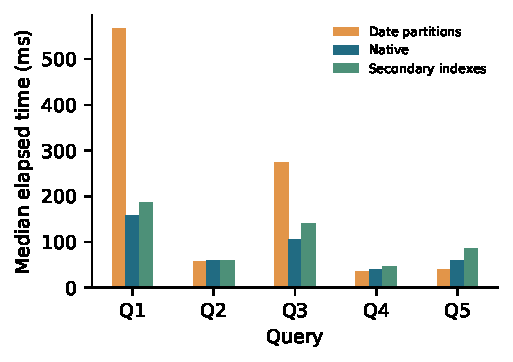
\includegraphics[width=\columnwidth]{benchmarks.pdf}\caption{Physical strategies measured on identical logical results. Lower is better; three warm runs per bar.}\end{figure}
Date partitions reduce Q5's median from 59.7 to 40.1 ms, while the full-month Q1 rises from 157.6 to 567.8 ms. Q4 also benefits modestly. Secondary indexes do not consistently help these scan-and-aggregate workloads. Index construction took 5.31 s and partition export took 1.80 s; these preparation costs are not hidden inside the timed SELECTs.
The evidence supports a workload-specific choice: keep native storage for broad analytical scans, and consider date partitions for narrow date slices and portable data access. Secondary indexes are not justified merely because they exist; their overhead and optimizer choices must be measured. These observations do not prove a universal optimum. A more rigorous final-stage study should randomize strategy order, increase repetitions, isolate resource contention, and evaluate concurrent and cold-cache workloads.

\section{Preliminary Mining Pipeline}
\subsection{Session feature engineering and temporal splits}
A warehouse-derived row per visit contains 18 features: event count; distinct products and categories; view/cart/purchase counts; price mean and standard deviation; gap mean and standard deviation; duration; transitions per minute; repeated-same-second rate; brand/category missingness rates; cart/purchase event rates; and category entropy $-\sum_c p_c\log p_c$. Count, duration, gap, price, and velocity features receive \code{log1p}; a StandardScaler is fit only on training rows. Rates and entropy are standardized without the log transform. Feature names and fitted transforms are stored with each model.

Training uses visits fully before October 22 (839,683), validation uses visits from October 22 fully before October 25 (121,241), and test starts October 25 (264,879). Twenty-nine visits crossing a split boundary are excluded from model fitting/evaluation. October itself is the available observation window, so month-edge truncation remains possible. Session-level splitting prevents one visit from leaking across periods, but users may recur; user IDs are not model features. This is a temporal operational scenario, not a new-user generalization experiment.

\subsection{Anomaly baseline and clustering}
Isolation Forest uses 100 trees, samples of 256, two jobs, and seed 544. It fits training sessions without labels; higher negative decision scores indicate more unusual feature combinations. The training 99.5th score percentile defines the review threshold. A simple velocity baseline uses the training 99.5th velocity percentile with a strict greater-than rule to avoid declaring all tied observations anomalous.

The final Isolation Forest flags 1,139/264,879 test visits (0.430\%) at threshold 0.6277. The velocity baseline flags 1,046 test visits above 12.0 transitions/minute. These counts compare review workload, not fraud detection accuracy. The selected clustering has $k=5$, validation silhouette 0.290, and test silhouette 0.296.
MiniBatch K-Means is fit on training sessions for $k\in\{3,4,5,6\}$, batch size 4,096, three initializations, and seed 544. Selection maximizes validation silhouette on a fixed random sample of 2,000 validation visits. The selected model is evaluated on 2,000 independently sampled test visits. Silhouette is in $[-1,1]$; a positive result indicates geometric separation under the chosen transformation, not verified fraud or a definitive customer taxonomy.

\begin{table}[t]\centering\caption{Held-out session profiles for the selected clustering}\label{tab:clusters}\scriptsize
\begin{tabular}{rrrrrr}\toprule Cluster & Visits & Events & Products & Duration(s) & Purchase share$^a$\\\midrule
0 & 97,897 & 1.0 & 1.0 & 0.0 & 0.000 \\
1 & 50,603 & 9.0 & 5.4 & 513.5 & 0.002 \\
2 & 32,443 & 11.1 & 7.9 & 684.0 & 0.003 \\
3 & 18,629 & 5.5 & 1.8 & 307.5 & 0.210 \\
4 & 65,307 & 2.5 & 1.7 & 92.6 & 0.000 \\
\bottomrule\end{tabular}\begin{flushleft}\scriptsize $^a$Mean within-visit purchase-event fraction, not visit conversion. Means are descriptive; labels below are interpretations.\end{flushleft}\end{table}
Cluster 0 consists of singleton visits. Clusters 1 and 2 contain longer, multi-product browsing, with cluster 2 exploring more products on average. Cluster 3 has the highest purchase-event fraction and fewer distinct products; cluster 4 represents brief browsing. These descriptive names are interpretations of aggregate profiles, not verified intent. The highest mean anomaly-flag rate occurs in cluster 2, but this alone does not validate the proposal's cluster-relative anomaly hypothesis.
The 100 highest-scoring test sessions are exported to a review queue with blank human labels and notes. No analyst review is claimed. Alert rates, cluster profiles, and review candidates are appropriate preliminary outputs; precision, recall, or fraud capture rates cannot be measured on REES46 without independently validated outcomes. The proposal's cluster-relative anomaly hypothesis and deeper models remain final-phase extensions.

\subsection{Labeled credit-card experiment}
The card feature matrix contains V1--V28 and \code{log1p(Amount)}. Time determines ordering and is excluded from the predictors; Class appears only as a target. Approximately 60/20/20 chronological splits preserve timestamp ties: training contains 170,882 rows/360 frauds (elapsed 0--120,395 s); validation 56,963/57 (120,396--145,247 s); test 56,962/75 (145,248--172,792 s). The scaler is trained only on training data. The original provider performed PCA; its fitting procedure cannot be audited here. Class prevalence changes between periods.

Four models/baselines are evaluated: amount-only ranking; unsupervised Isolation Forest (100 trees, 256 samples); balanced logistic regression (maximum 1,000 iterations); and a supervised Random Forest (100 trees, maximum depth 12, minimum leaf size 2, balanced-subsample class weights). The supervised methods have access to training labels; their superiority is not an equal-information comparison with the unsupervised methods. Isolation Forest training does not remove known frauds using labels.

For each model, the decision threshold maximizes validation F1 and is then frozen before test evaluation. Test scores are reported once using average precision (AP), ROC-AUC, precision, recall, F1, and confusion counts. AP summarizes the precision--recall curve and is not the trapezoidal PR area. The no-skill test AP is the test prevalence, approximately 0.00132. No oversampling or test-set threshold optimization is applied.

\begin{table}[t]\centering\caption{Chronological credit-card test results}\label{tab:card}\scriptsize
\begin{tabular}{lrrrrr}\toprule Model & AP & ROC-AUC & Precision & Recall & F1\\\midrule
Isolation Forest & 0.048 & 0.952 & 0.069 & 0.360 & 0.116 \\
Logistic regression & 0.747 & 0.982 & 0.961 & 0.653 & 0.778 \\
Random Forest & 0.812 & 0.961 & 0.891 & 0.760 & 0.820 \\
Amount baseline & 0.001 & 0.382 & 0.003 & 0.040 & 0.005 \\
\bottomrule\end{tabular}\end{table}
\begin{figure}[t]\centering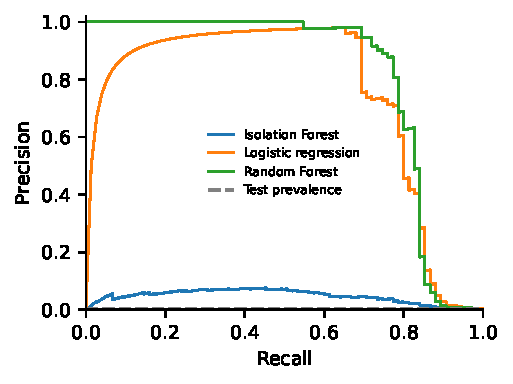
\includegraphics[width=\columnwidth]{pr.pdf}\caption{Precision--recall curves on the untouched chronological card test set. The dashed prevalence baseline is close to zero.}\end{figure}
Random Forest produces 57 true positives, 7 false positives, 18 false negatives and 56,880 true negatives. Logistic regression is more precise at its selected operating point but misses more frauds (49 true positives, 26 false negatives). Isolation Forest has high ROC-AUC but AP only 0.048 and 363 false positives at its selected threshold; ROC-AUC alone would conceal this burden. The amount baseline performs poorly and does not validate amount as a useful standalone fraud rule.

A 100-replicate stratified bootstrap on the fixed test set gives percentile 95\% AP intervals of 0.038--0.062 for Isolation Forest, 0.625--0.845 for Logistic regression, 0.720--0.883 for Random Forest. These conditional intervals hold test class counts fixed and assume independent resampling within each class. They do not incorporate training variability, entity dependence, or future distribution shift; overlapping intervals do not establish a statistically significant ordering between the supervised models. Only 75 test frauds are available.

\section{Reproducibility, Limitations, and Remaining Work}
The package contains the source manifest, SQL DDL, all five queries, Airflow DAG, sequential pipeline, pinned analytical dependencies, trained models, measured result tables and plans, quality checks, test transcript, report source, and a read-only demo script. A database snapshot accompanies the project for an immediate live demonstration. Full reproduction downloads the two original datasets and reruns the pipeline; the live demo can query the snapshot without rerunning training. Raw data, virtual environments, Airflow credentials/metadata DB, and temporary spill files are excluded from the package.

The recorded DAG execution is successful and the code demonstration is prepared, but an in-person live presentation has not occurred. The supplied demo script walks through source grains, SCD history, quality gates, OLAP queries, timing comparisons, cluster profiles, and card baselines. 

Material limitations are the one-month sampled clickstream, observed rather than authoritative SCD changes, no e-commerce fraud labels, only two days of card data, unavailable entity linkage, a small test fraud count, possible duplicate dependence, and single-host performance. No purchase-event value is presented as actual sales revenue. The Phase 1 PostgreSQL deployment, distributed scale-out, autoencoder/HDBSCAN experiments, cluster-relative anomaly testing, and analyst adjudication are not reported as completed.

For the final phase, priorities are independently labeling a review sample; evaluating duplicate and feature ablations; adding group-aware or repeated temporal validation if identifiers/data become available; quantifying model drift and alert workload; broadening performance experiments; and testing containerized deployment. These steps extend the completed Phase 2 warehouse and preliminary mining results without overstating their current evidence.

\begin{thebibliography}{9}
\bibitem{assignment} Mahidol University, ``ITCS544 Term Project Assignment,'' Term 1, 2026, pp. 1--3. Supplied course brief.
\bibitem{rees} REES46, ``Public datasets: marketplace October 2019,'' \url{https://data.rees46.com/}, accessed Oct. 12, 2026.
\bibitem{ulb} ULB Machine Learning Group and Worldline, ``Credit Card Fraud Detection,'' \url{https://www.kaggle.com/datasets/mlg-ulb/creditcardfraud}, accessed Oct. 12, 2026.
\bibitem{tf} TensorFlow, ``Classification on imbalanced data,'' \url{https://www.tensorflow.org/tutorials/structured_data/imbalanced_data}, dataset provenance and download mirror, accessed Oct. 12, 2026.
\bibitem{proposal} K. C. T. Byin, C. Ou, and A. M. Myat, ``ITCS544 Phase 1 Proposal: Fraud Detection,'' supplied project proposal, 2026.
\end{thebibliography}
\end{document}
